\section{Motivation}
\subsection{Application Results}



%%%%%%%%%%%%%%%%%%%%%%%%%%%%%%%%%%%%%%%%%%%%%%%%%
\frame
{
  \Large
  \begin{block}{}
    \center{Results from Physics Applications built}
    \center{on top of \bf{\libmesh{}}}
  \end{block}
}



%%%%%%%%%%%%%%%%%%%%%%%%%%%%%%%%%%%%%%%%%%%%%%%%%
\frame
{
  \frametitle{Compressible Navier-Stokes}
  \begin{center}
    \only<1>{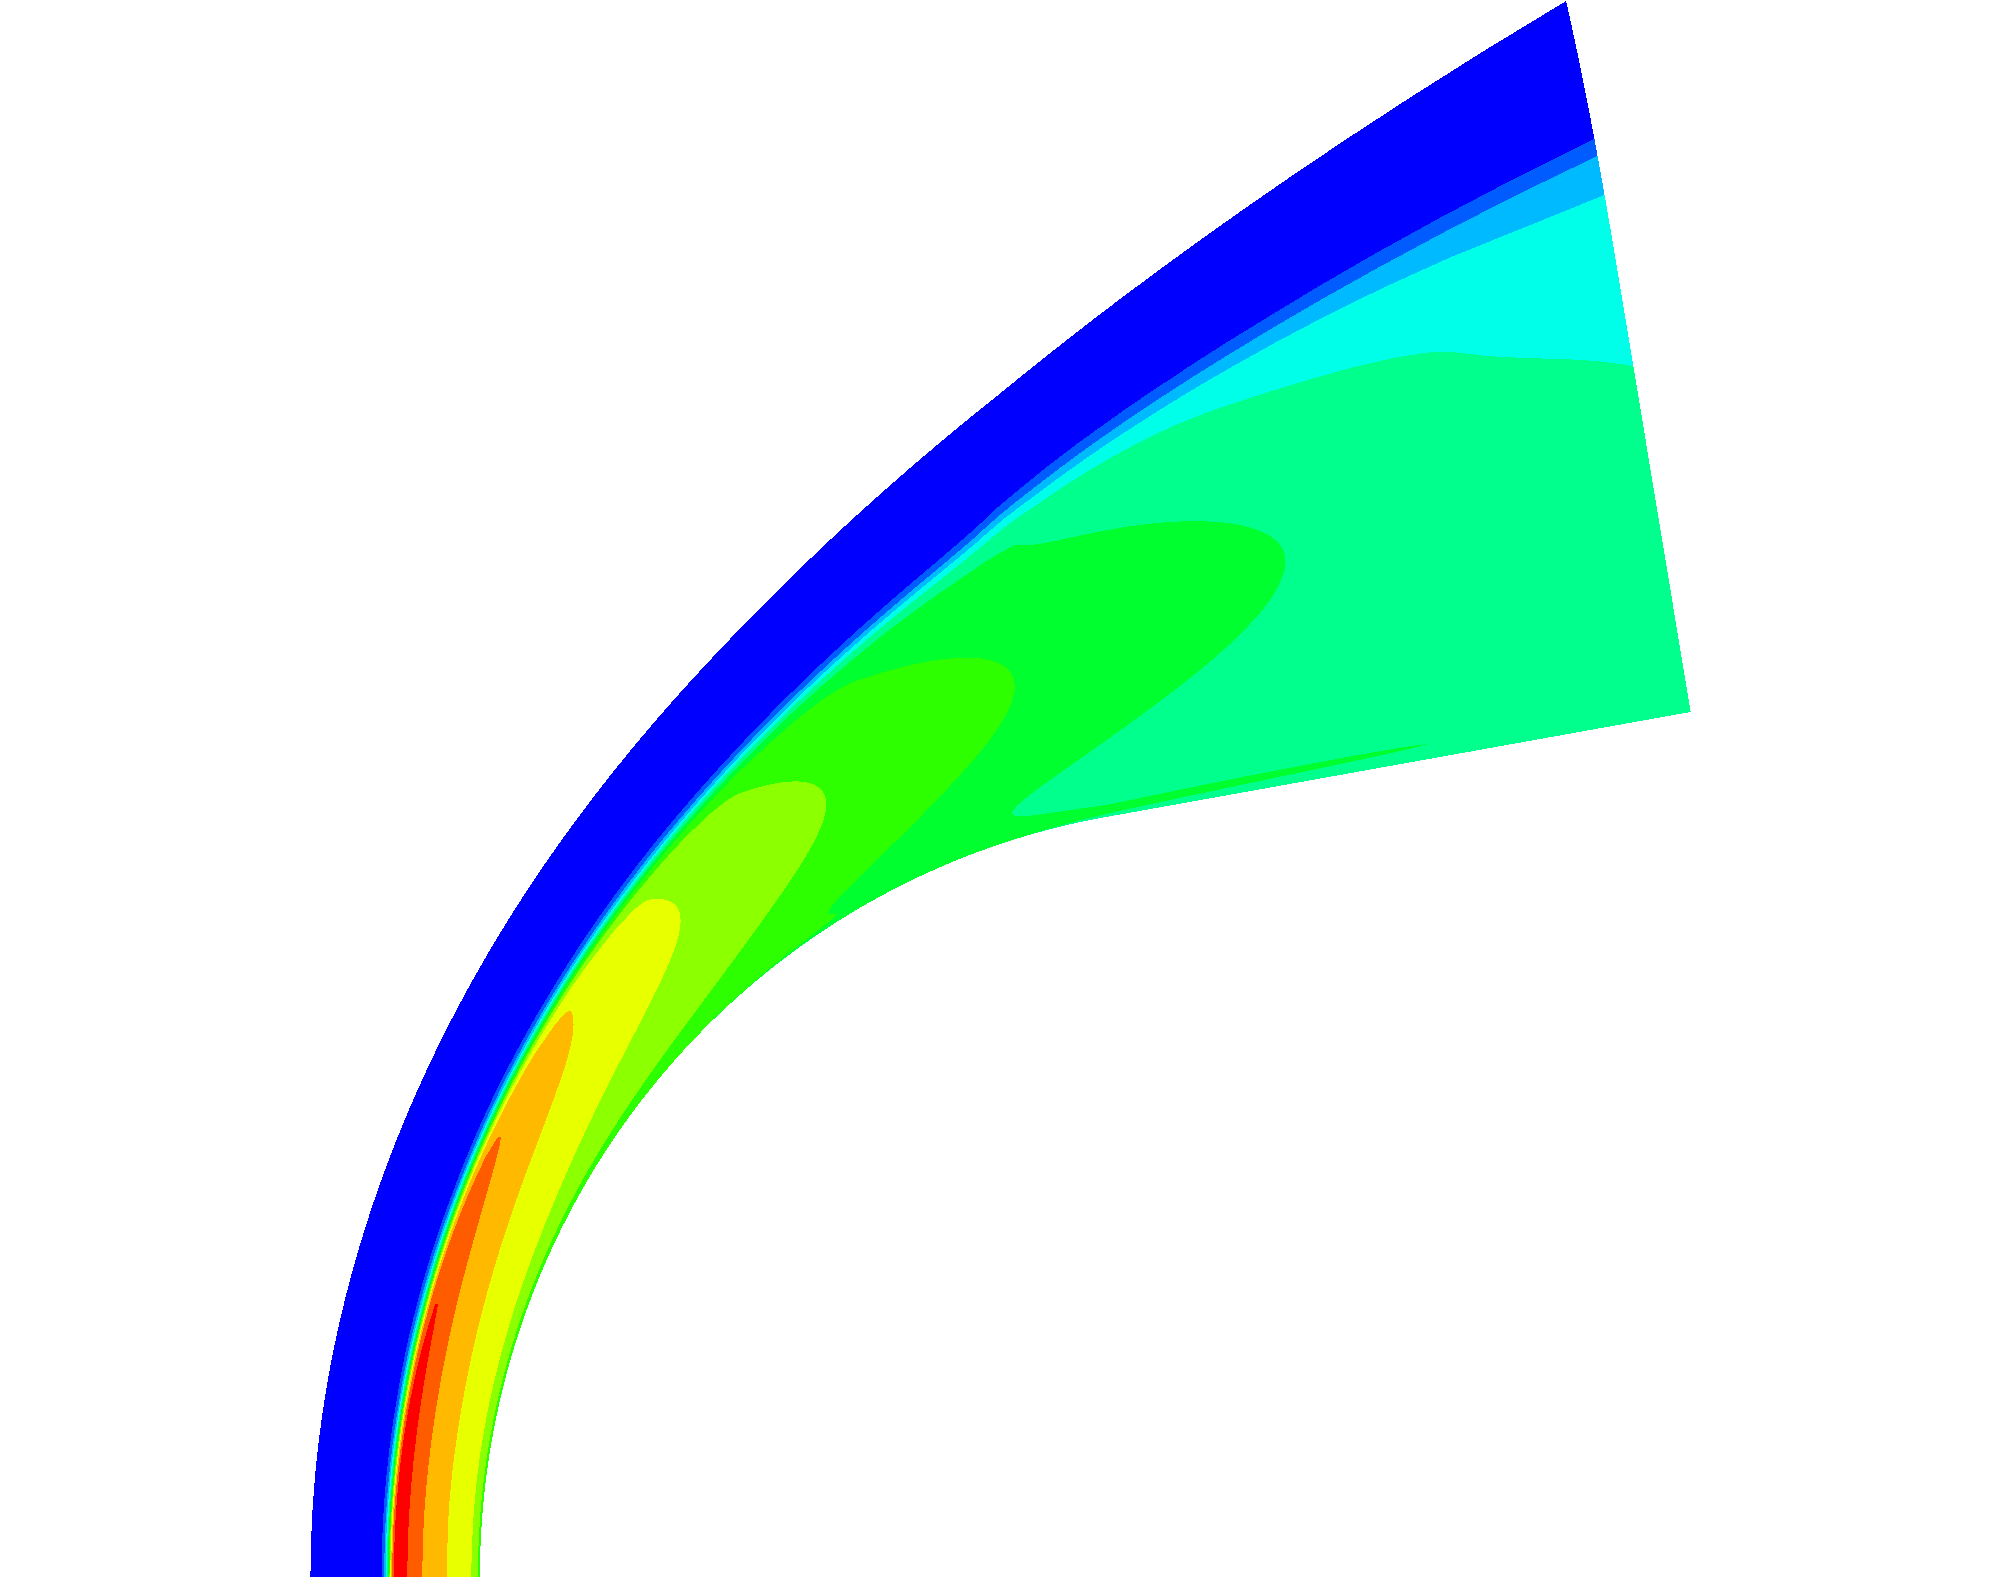
\includegraphics[height=0.9\textheight]{nosetip/smeared.png}}

    \only<2>{\includegraphics[height=0.9\textheight]{nosetip/amr.png}}

    \only<3>{\includegraphics[height=0.9\textheight]{nosetip/smeared.pdf}}

    \only<4>{\includegraphics[height=0.9\textheight]{nosetip/amr.pdf}}

  \end{center}
}
%===============================================================================
% NEW SLIDE
%===============================================================================
\frame
{
  \frametitle{Arcjet Nozzle Calculation}
  \begin{center}

    \only<1>{\includegraphics[width=0.95\linewidth,trim=4px 4px 4px 4px,clip]{arcjet/viz/T}}

    \only<2>{\includegraphics[width=0.95\linewidth,trim=4px 4px 4px 4px,clip]{arcjet/viz/M}}

  \end{center}
}



%===============================================================================
% NEW SLIDE
%===============================================================================
\frame
{
  \frametitle{Arcjet Nozzle Calculation}
  \begin{center}

    \only<1>{\includegraphics[width=.95\textwidth,trim=4px 4px 4px 4px,clip]{arcjet/data/nozzle/P-streamlines.png}}

    \only<2>{\includemovie[autoplay,loop,text={\includegraphics[width=.95\textwidth,trim=4px 4px 4px 4px,clip]{arcjet/data/nozzle/P-streamlines.png}}]{.95\textwidth}{}{rawfigs/arcjet/data/nozzle/P.avi}}

  \end{center}
}



%===============================================================================
% NEW SLIDE
%===============================================================================
\frame
{
  \frametitle{Coupled Pyrolysis, Temperature}
  \begin{center}

    \only<1>{\includegraphics[height=.85\textheight]{arcjet/data/coupled/T.png}}

    \only<2>{\includemovie[autoplay,loop,text={\includegraphics[height=.85\textheight]{arcjet/data/coupled/T.png}}]{}{.85\textheight}{rawfigs/arcjet/data/coupled/T.avi}}

  \end{center}
}


%===============================================================================
% NEW SLIDE
%===============================================================================
\frame
{
  \frametitle{Coupled Pyrolysis, Pyrolysis gas mass flux, $\dot{m}$}
  \begin{center}

    \only<1>{\includegraphics[height=.85\textheight]{arcjet/data/coupled/mdotzoom.png}}

    \only<2>{\includemovie[autoplay,loop,text={\includegraphics[height=.85\textheight]{arcjet/data/coupled/mdotzoom.png}}]{}{.85\textheight}{rawfigs/arcjet/data/coupled/mdotzoom.avi}}

  \end{center}
}



\frame
{
  \frametitle{Coupled Thermal/Solid Mechanics}
  \begin{center}

    \only<1>{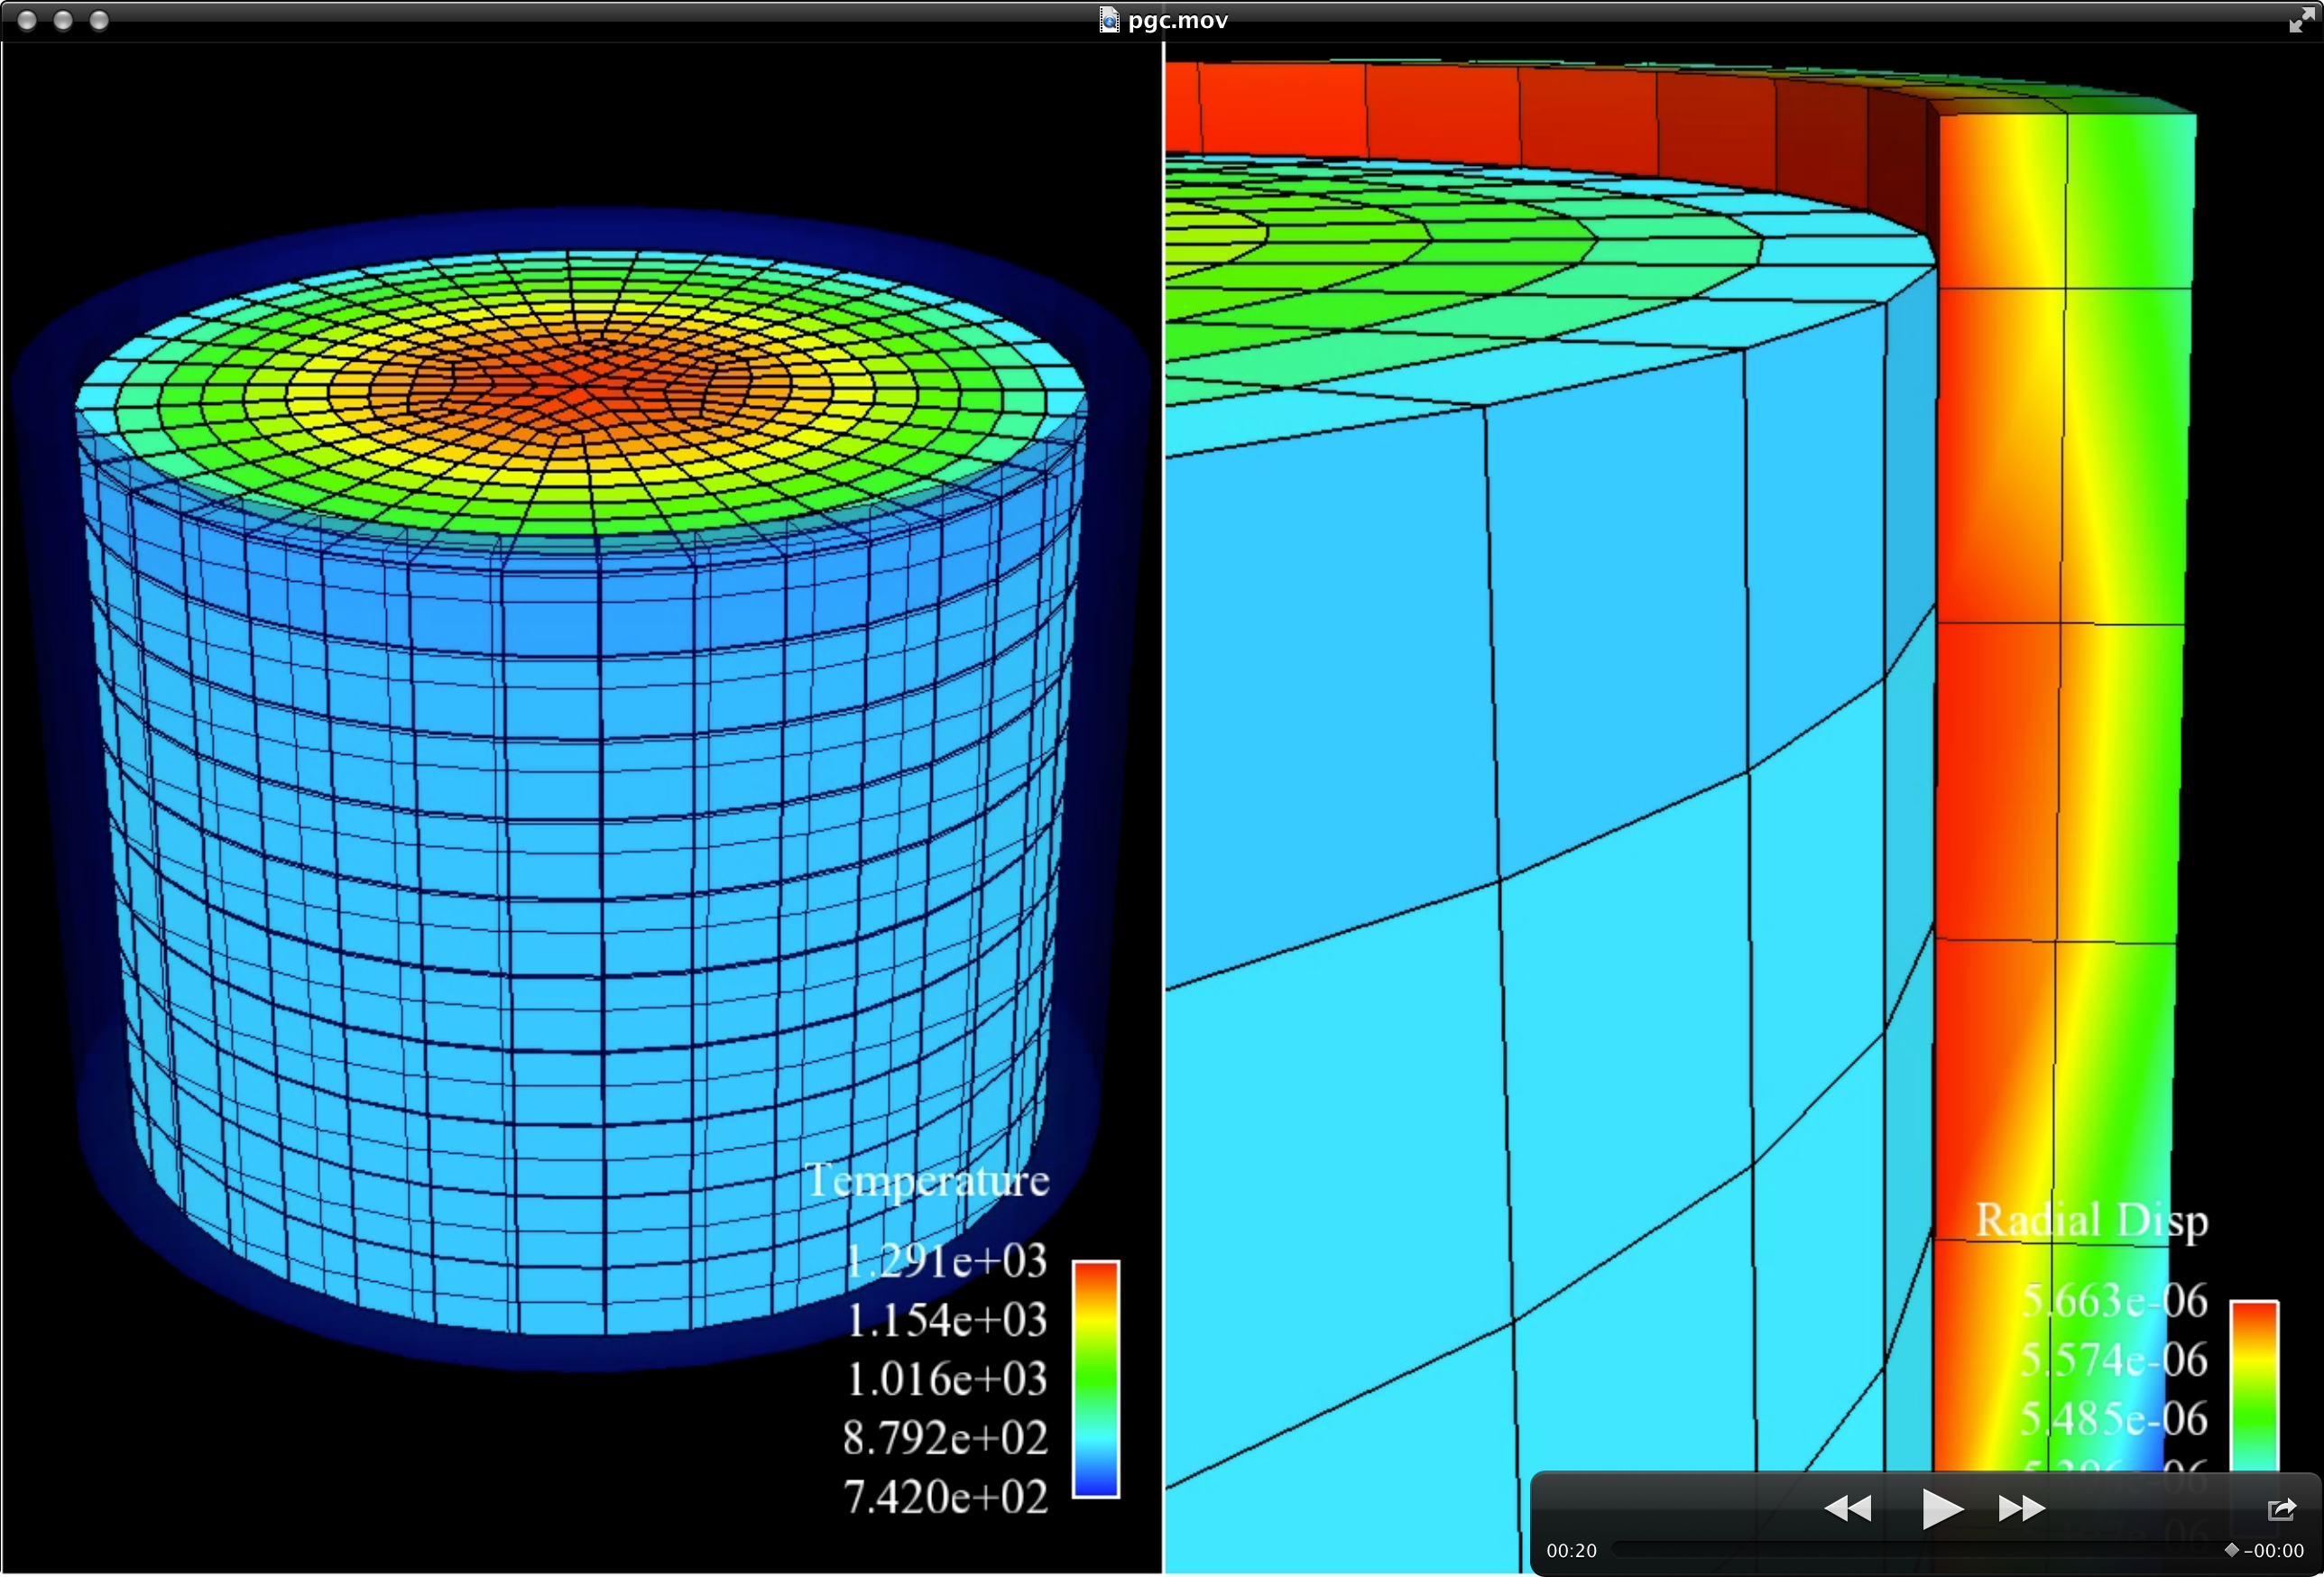
\includegraphics[height=.85\textheight]{Gaston/pgc.png}}

    %\only<2>{\includemovie[autoplay,loop,text={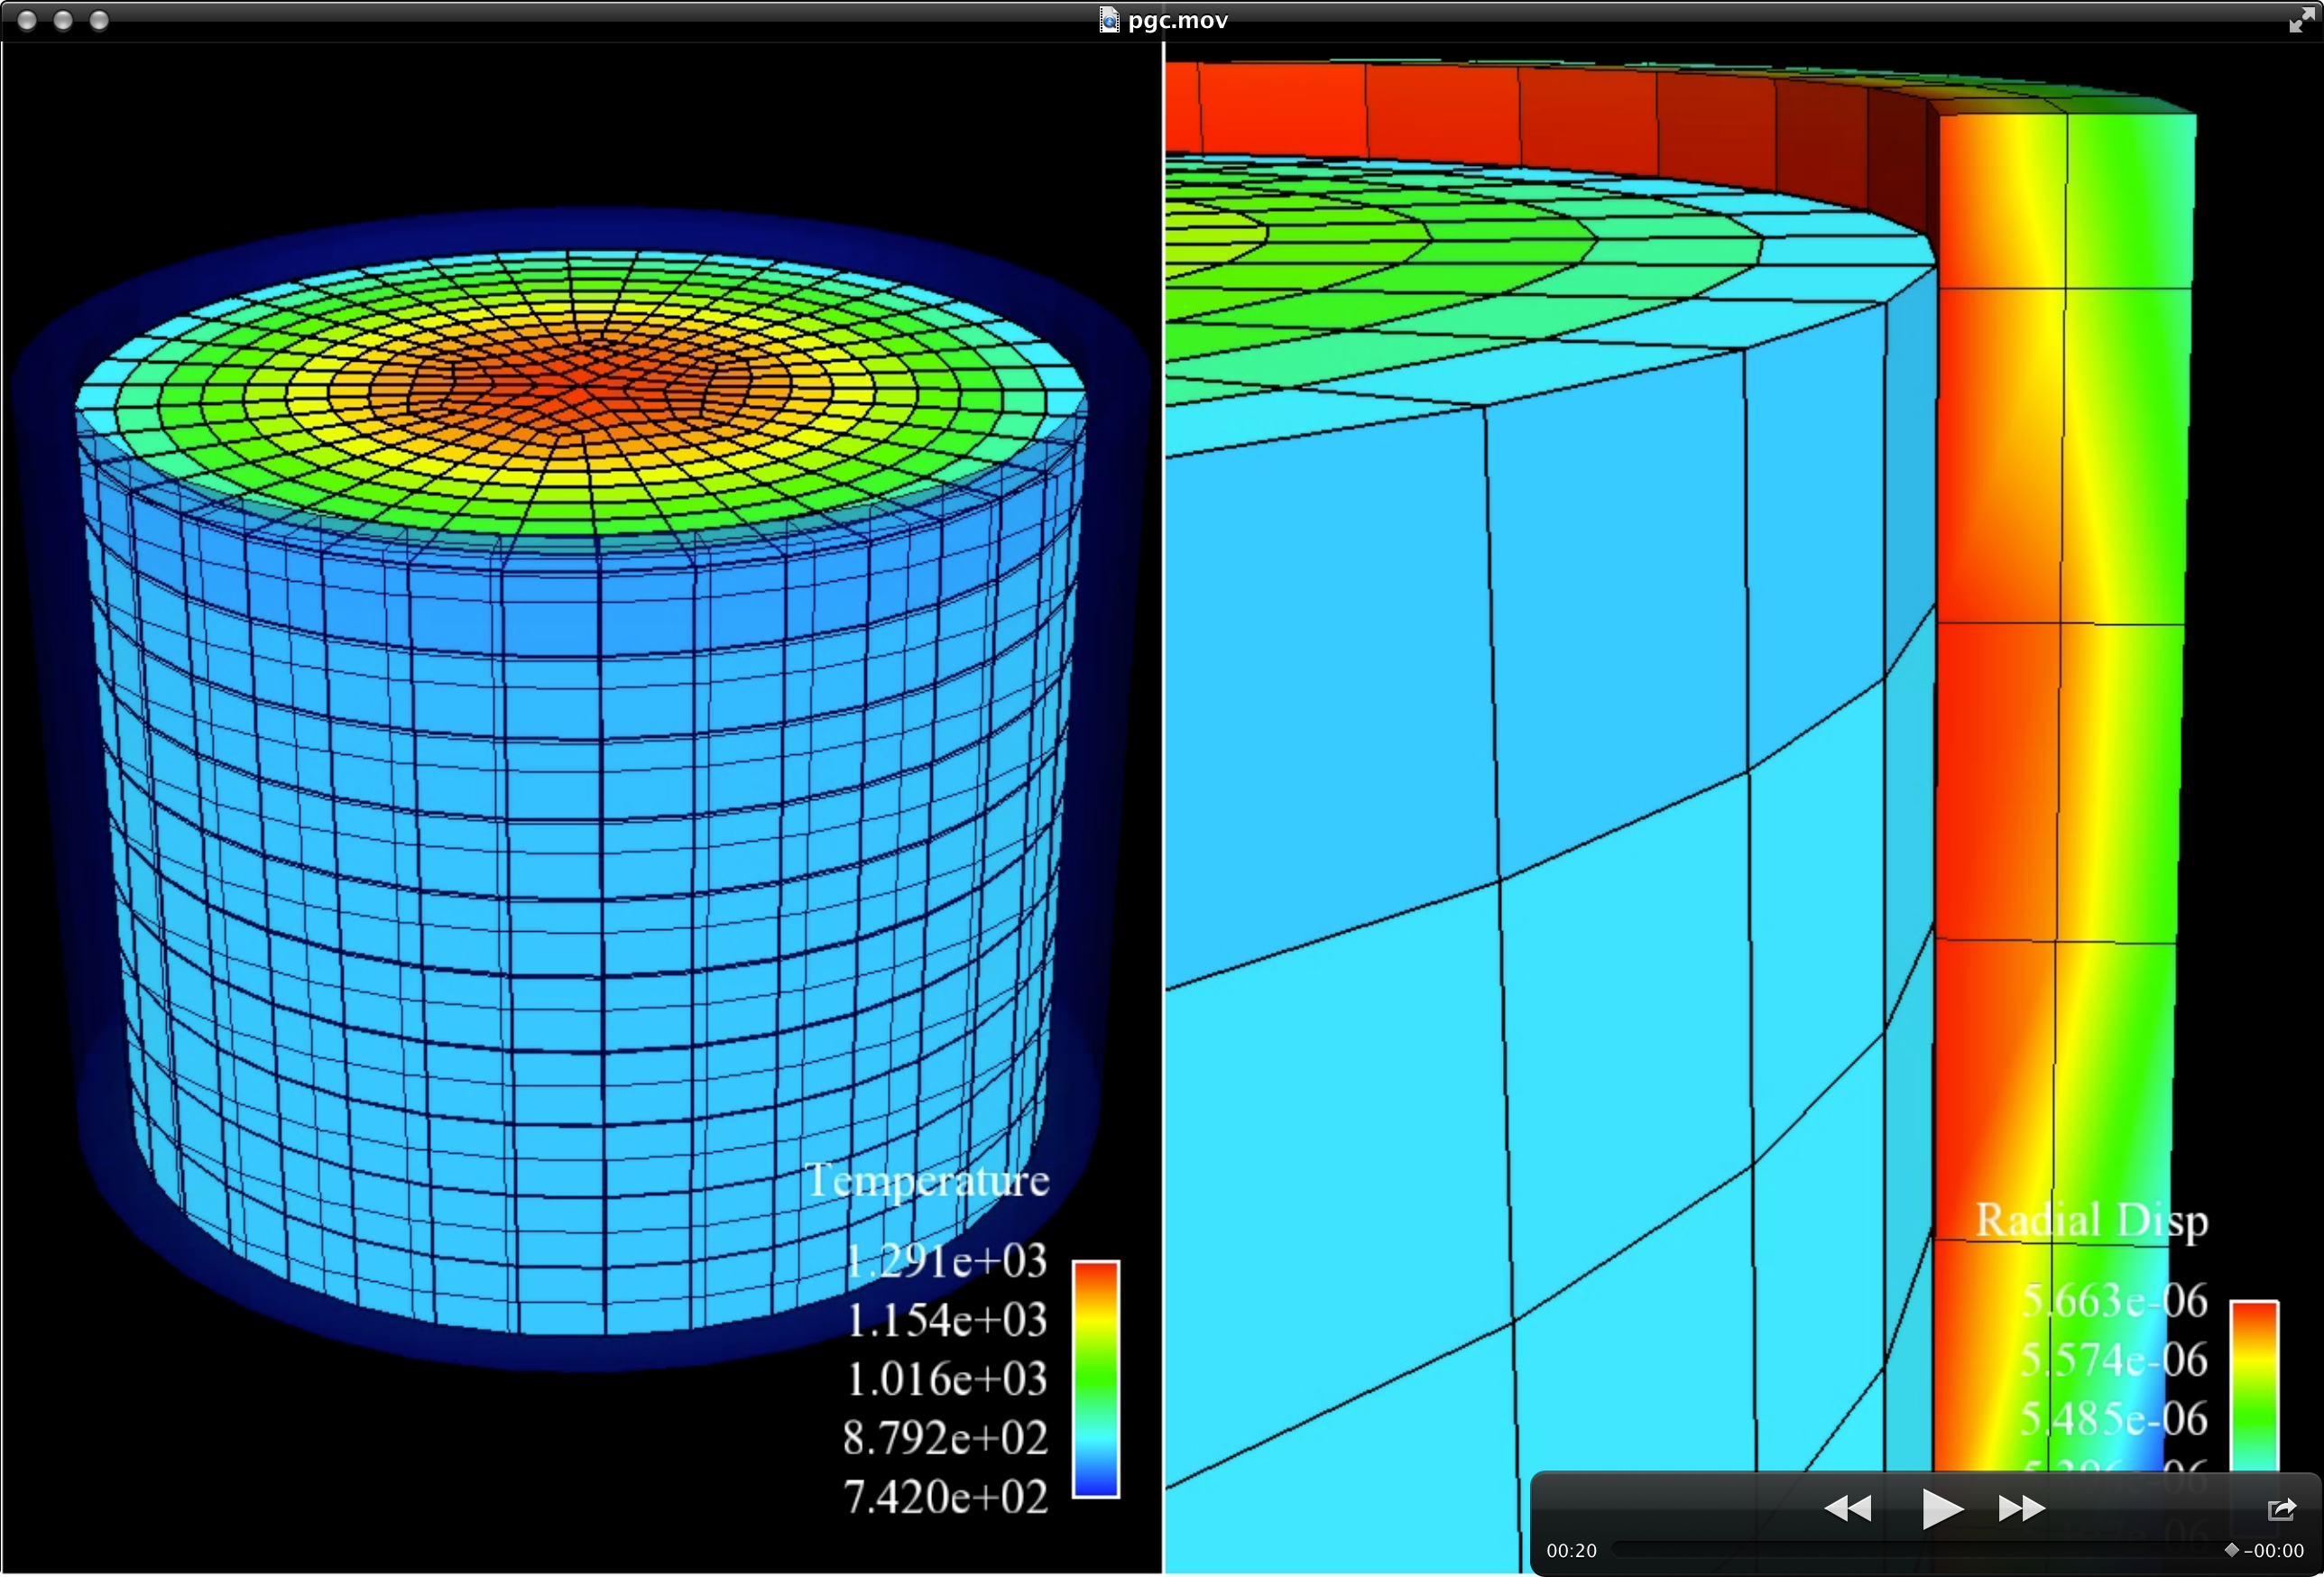
\includegraphics[height=.85\textheight]{Gaston/pgc.png}}]{}{.85\textheight}{Gaston/pgc.avi}}

  \end{center}
}



\frame
{
  \frametitle{The MOOSE Framework - Gaston et al., INL}
  \begin{center}
    \fbox{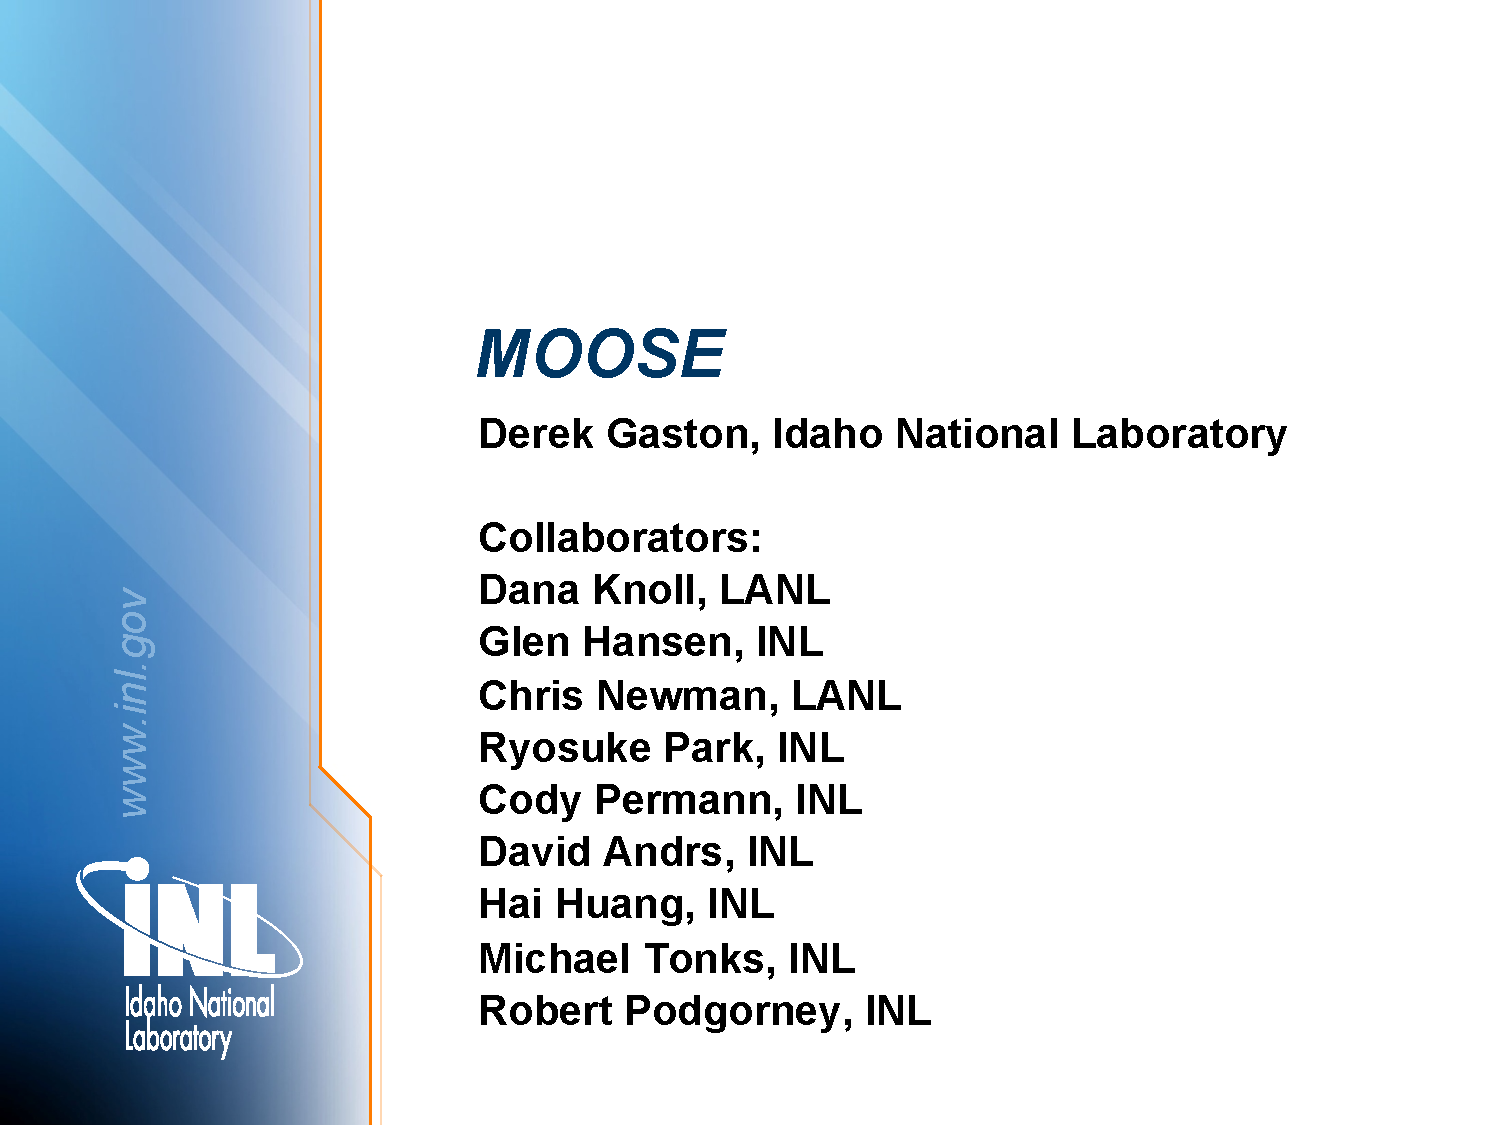
\includegraphics[page=1,height=0.8\textheight]{Gaston/talk}}
  \end{center}
}



\frame
{
  \frametitle{The MOOSE Framework - Gaston et al., INL}
  \begin{center}
    \fbox{\includegraphics[page=2,height=0.8\textheight]{Gaston/talk}}
  \end{center}
}



\frame
{
  \frametitle{The MOOSE Framework - Gaston et al., INL}
  \begin{center}
    \fbox{\includegraphics[page=4,height=0.8\textheight]{Gaston/talk}}
  \end{center}
}



\frame
{
  \frametitle{The MOOSE Framework - Gaston et al., INL}
  \begin{center}
    \fbox{\includegraphics[page=22,height=0.8\textheight]{Gaston/talk}}
  \end{center}
}



\frame
{
  \frametitle{The MOOSE Framework - Gaston et al., INL}
  \begin{center}
    \large
    \vspace{2em}

    Especially if you want to use Jacobian-Free Newton-Krylov solution techniques, consider acessing \libmesh{} through MOOSE:
    \vspace{1em}

    \url{http://mooseframework.org}
  \end{center}
}
